%%%%%%%%%%%%%%%%%%%%%%%%%%%%%%%%%%%%%%%%%
% Sullivan Business Report
% LaTeX Template
% Version 1.0 (May 5, 2022)
%
% This template originates from:
% https://www.LaTeXTemplates.com
%
% Author:
% Vel (vel@latextemplates.com)
%
% License:
% CC BY-NC-SA 4.0 (https://creativecommons.org/licenses/by-nc-sa/4.0/)
%
%%%%%%%%%%%%%%%%%%%%%%%%%%%%%%%%%%%%%%%%%


%----------------------------------------------------------------------------------------
%	CLASS, PACKAGES AND OTHER DOCUMENT CONFIGURATIONS
%----------------------------------------------------------------------------------------

\documentclass[
    a4paper, % Paper size, use either a4paper or letterpaper
	12pt, % Default font size, the template is designed to look good at 12pt so it's best not to change this
	%unnumberedsections, % Uncomment for no section numbering
    ]{CSSullivanBusinessReport}
    
    \addbibresource{sample.bib} % BibLaTeX bibliography file

%----------------------------------------------------------------------------------------
%	REPORT INFORMATION
%----------------------------------------------------------------------------------------

\reporttitle{CPE 233 Hardware Assignment 1} % The report title is to appear on the title page and page headers, do not create manual new lines here as this will carry over to page headers

\reportsubtitle{Reverse Engineering and Testing ROM} % Report subtitle, include new lines if needed

\reportauthors{Report by:\\\smallskip Ethan Vosburg (evosburg@calpoly.edu)} % Report authors/group/department, include new lines if needed

\reportdate{\today} % Report date, include new lines for additional information if needed

\rightheadercontent{
\includegraphics[width=3cm]{creodocs_logo.pdf}} % The content in the right header, you may want to add your own company logo or use your company/department name or leave this command empty for no right header content

%----------------------------------------------------------------------------------------

\begin{document}

%----------------------------------------------------------------------------------------
%	TITLE PAGE
%----------------------------------------------------------------------------------------

\thispagestyle{empty} % Suppress headers and footers on this page

\begin{fullwidth} % Use the whole page width
	\vspace*{-0.075\textheight} % Pull logo into the top margin
	
	\hfill
\includegraphics[width=5cm]{creodocs_logo.pdf} % Company logo

	\vspace{0.15\textheight} % Vertical whitespace

	\parbox{0.9\fulltextwidth}{\fontsize{50pt}{52pt}\selectfont\raggedright\textbf{\reporttitle}\par} % Report title, intentionally at less than full width for nice wrapping. Adjust the width of the \parbox and the font size as needed for your title to look good.
	
	\vspace{0.03\textheight} % Vertical whitespace
	
	{\LARGE\textit{\textbf{\reportsubtitle}}\par} % Subtitle
	
	\vfill % Vertical whitespace
	
	{\Large\reportauthors\par} % Report authors, group or department
	
	\vfill\vfill\vfill % Vertical whitespace
	
	{\large\reportdate\par} % Report date
\end{fullwidth}

\newpage

%----------------------------------------------------------------------------------------
%	DISCLAIMER/COPYRIGHT PAGE
%----------------------------------------------------------------------------------------

% \thispagestyle{empty} % Suppress headers and footers on this page

% \begin{twothirdswidth} % Content in this environment to be at two-thirds of the whole page width
% 	\footnotesize % Reduce font size
	
% 	\subsection*{Disclaimer}

% 	Lorem ipsum dolor sit amet, consectetur adipiscing elit. Praesent porttitor arcu luctus, imperdiet urna iaculis, mattis eros. Pellentesque iaculis odio vel nisl ullamcorper, nec faucibus ipsum molestie. Sed dictum nisl non aliquet porttitor. Etiam vulputate arcu dignissim, finibus sem et, viverra nisl. Aenean luctus congue massa, ut laoreet metus ornare in. Nunc fermentum nisi imperdiet lectus tincidunt vestibulum at ac elit.
	
% 	\subsection*{Copyright}
	
% 	\textcopyright~[Year] [Company] 
	
% 	Copyright notice text\ldots In hac habitasse platea dictumst. Curabitur mattis elit sit amet justo luctus vestibulum. In hac habitasse platea dictumst. Pellentesque lobortis justo enim, a condimentum massa tempor eu. Ut quis nulla a quam pretium eleifend nec eu nisl. Nam cursus porttitor eros, sed luctus ligula convallis quis.
	
% 	\subsection*{Contact}
	
% 	Address Line 1\\
% 	Address Line 2\\
% 	Address Line 3
	
% 	Business Number 123456
	
% 	Contact: name@company.com
	
% 	\vfill % Push the following down to the bottom of the page
	
% 	\subsubsection*{Changelog}
	
% 	\scriptsize % Reduce font size further
	
% 	\begin{tabular}{@{} L{0.05\linewidth} L{0.15\linewidth} L{0.6\linewidth} @{}} % Column widths specified here, change as needed for your content
% 		\toprule
% 		v1.0 & 20XX-02-05 & Lorem ipsum dolor sit amet, consectetur adipiscing elit. Praesent porttitor arcu luctus, imperdiet urna iaculis, mattis eros.\\
% 		v1.1 & 20XX-02-27 & Pellentesque iaculis odio vel nisl ullamcorper, nec faucibus ipsum molestie.\\
% 		v1.2 & 20XX-03-15 & Sed dictum nisl non aliquet porttitor.\\
% 		\bottomrule
% 	\end{tabular}
% \end{twothirdswidth}

% \newpage

%----------------------------------------------------------------------------------------
%	TABLE OF CONTENTS
%----------------------------------------------------------------------------------------
\bigskip
\begin{twothirdswidth} % Content in this environment to be at two-thirds of the whole page width
	\tableofcontents % Output the table of contents, automatically generated from the section commands used in the document
\end{twothirdswidth}

\newpage

%----------------------------------------------------------------------------------------
%	SECTIONS
%----------------------------------------------------------------------------------------
\begin{fullwidth} % Use the whole page width

\section{Project Description} % Top level section

Reverse engineer the excerpts from the \verb|otter_memory.mem| file is shown below to determine the assembly instructions implemented by this file. This can be done by first creating a table similar to Table 1 from the Example Program. Any other lines from this file can be assumed to be all zeros and disregarded. 

\section{Reverse Engineering} % Second level section

\subsection{Reverse Engineering Table} % Third level section
Below is a table of the machine code and assembly instructions from the \verb|otter_memory.mem| file. The machine code was converted to binary and then to assembly instructions. By converting to binary the structure of instruction could be more easily seen and then specific instructions could be identified and then converted to assembly instructions. The assembly instructions were then written in the table. To verify the assembly instructions, once the assembly was written, it was recompiled and the compared to the original memory file. The assembly instructions were correct and the program was able to be run.

\begin{table}[ htbp]
    \centering
    % \captionsetup{justification=centering}
    \footnotesize
    \captionsetup{style=widetable}
    \caption{Machine Code to Instruction Table}
    \begin{tabular}{|c|c|c|c|}
    % \begin{tabular}{|c|c|}
    \hline
    Address & Machine Code (Hex) & Machine Code (Binary) & Assembly Instruction  \\
    \hline
    \hline
        0000 & 11000537 & 00010001000000000000010100110111 & lui x10, 69632      \\
        \hline
        0004 & 00a00f13 & 00000000101000000000111100010011 & addi x30, x0, 10    \\
        \hline
        0008 & 00051783 & 00000000000001010001011110000011 & jump:lh x15, 0(x10) \\
        \hline
        000C & 41e7da33 & 01000001111001111101101000110011 & sra x20, x15, x30   \\
        \hline
        0010 & 00fa4633 & 00000000111110100100011000110011 & xor x12, x20, x15   \\
        \hline
        0014 & 04c52023 & 00000100110001010010000000100011 & sw x12, 64(x10)     \\
        \hline
        0018 & ff1ff06f & 11111111000111111111000001101111 & jal x0, jump        \\
    \hline
    \end{tabular}
    \label{tab:machineToInstruction}
\end{table}


\subsection{Reversed Engineered Program} % Third level section

Below is the reverse-engineered program from the \verb|otter_memory.mem| file. The program is a simple loop that shifts the value in \verb|x15| right by the value in \verb|x30|, exclusive ors the result with the original value in \verb|x15|, and then stores the result in \verb|x12| and loops.

\captionsetup{style=widetable}
\begin{lstlisting}[caption=Assembly instructions from reverse engineered file]
        lui     x10, 69632      // load upper immediate
        addi    x30, x0, 10     // add immediate
jump:       
        lh      x15, 0(x10)     // load halfword
        sra     x20, x15, x30   // shift right arithmetic
        xor     x12, x20, x15   // exclusive or
        sw      x12, 64(x10)    // store word
        jal     x0,  jump       // jump
\end{lstlisting}

\section{Testing rom} % Second level section

To create a more robust testbench, the \verb|ProgRom_TB| was created. This testbench reads in the \verb|otter_memory.mem| file and then compares the machine code instructions from the file to the machine code instructions from the \verb|ProgRom| module. Once iterating through all of the instructions an overall pass/fail is displayed. The testbench was able to be run and passed. The testbench is shown below.

\begin{lstlisting}[language=Verilog, caption=Verilog Testbench for ProgRom]
`timescale 1ns / 1ps
//////////////////////////////////////////////////////////////////////////////////
// Company: Cal Poly SLO
// Engineer: Ethan Vosburg
// 
// Create Date: 01/11/2024 10:40:40 PM
// Design Name: ProgRom Testbench
// Module Name: ProgRom_TB
// Project Name: HW1-ProgROM
// Target Devices: Basys 3
// Description: This is a testbench for the ProgRom module that takes in a mem file and checks that the program memory is correct
// 
// Revision: 1.0
// Revision 0.01 - File Created
// Additional Comments: Still need to work on dynamic array assignment
// 
//////////////////////////////////////////////////////////////////////////////////


module ProgRom_TB();
    // Inputs
    logic PROG_CLK_TB; // 1-bit clock
    logic [31:0] PROG_ADDR_TB; // 32-bit address

    // Outputs
    logic [31:0] INSTRUCT_TB; // 32-bit machine code instruction

    // Logic
    logic pass; // 1 = pass, 0 = fail

    // rom_TB type set up
    (* rom_style="{distributed | block}" *)
	(* ram_decomp = "power" *) logic [31:0] rom_TB [0:16383];

    // Instantiate the Unit Under Test (UUT)
    ProgRom uut (
        .PROG_CLK(PROG_CLK_TB), 
        .PROG_ADDR(PROG_ADDR_TB), 
        .INSTRUCT(INSTRUCT_TB)
    );

    // Begin simulation code
    initial begin
        // Initialize Logic
        PROG_CLK_TB = 0; // Initialize PROG_CLK_TB
        pass = 1; // Initialize pass to 1
        
        $readmemh("otter_memory.mem", rom_TB , 0, 16383); // Read in otter_memory.mem file

        // Iterate through rom_TB and compare to INSTRUCT_TB
        // If there is a mismatch, set pass to 0
        // Note: the comparison is hardcoded to stop for this case
        for (int i = 0; i < 7; i++) begin
            PROG_ADDR_TB = 32'h0000_0000 + (i*4); // Request machine code instruction from address
            #20 // Wait for INSTRUCT_TB to be updated

            // Display values for debugging and verification
            $display("rom[%0d]: %h", i, INSTRUCT_TB);
            $display("rom_tb[%0d]: %h", i, rom_TB[i]);

            // Compare INSTRUCT_TB to rom_TB[i]
            if (INSTRUCT_TB == (32'h0000_0000 + rom_TB[i])) begin
                $display("Match rom_TB[%0d] = %h", i, rom_TB[i]);
            end else begin
                $display("No Match rom_TB[%0d] = %h", i, rom_TB[i]);
                pass = 0; // Do not allow the test to pass
            end
            #20;
        end

        // Display overall pass/fail
        if (pass == 1) begin
            $display("OVERALL PASS");
        end else begin
            $display("OVERALL FAIL");
        end 
    end

    // Toggle the clock
    always #5 PROG_CLK_TB = ~PROG_CLK_TB;
endmodule
\end{lstlisting}

% Shown here is the output from the testbench.
% \begin{figure}[htbp]
%     \centering
%     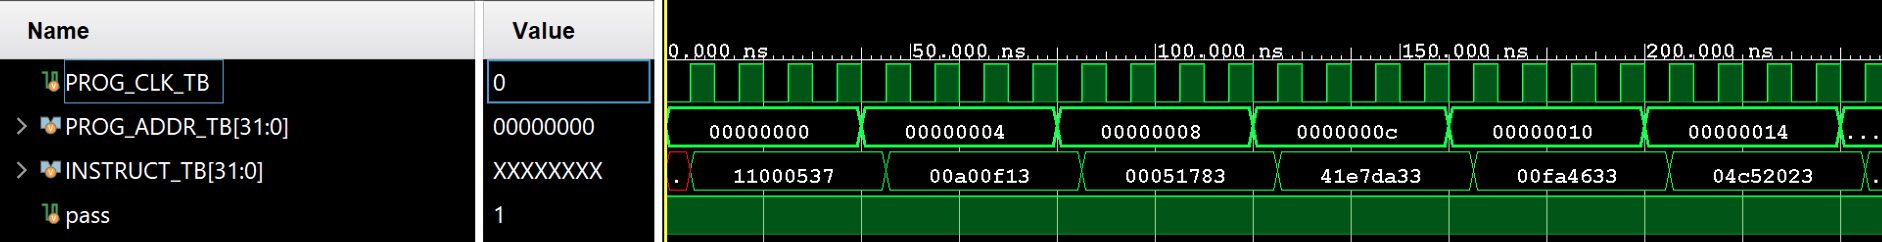
\includegraphics[width=.75\pdfpagewidth]{Figures/ProgRom Simulation.png}
%     \caption{ProgRom\_TB Output}
%     \label{fig:ProgRom_TB_Output}
% \end{figure}


% Running this program outputs the following:

\begin{lstlisting}[language=Verilog, caption=TCl Output from ProgRom\_TB]
rom[0]: 11000537
rom_tb[0]: 11000537
Match rom_TB[0] = 11000537
rom[1]: 00a00f13
rom_tb[1]: 00a00f13
Match rom_TB[1] = 00a00f13
rom[2]: 00051783
rom_tb[2]: 00051783
Match rom_TB[2] = 00051783
rom[3]: 41e7da33
rom_tb[3]: 41e7da33
Match rom_TB[3] = 41e7da33
rom[4]: 00fa4633
rom_tb[4]: 00fa4633
Match rom_TB[4] = 00fa4633
rom[5]: 04c52023
rom_tb[5]: 04c52023
Match rom_TB[5] = 04c52023
rom[6]: ff1ff06f
rom_tb[6]: ff1ff06f
Match rom_TB[6] = ff1ff06f
OVERALL PASS
\end{lstlisting}

\begin{figure}[htbp]
    \centering
    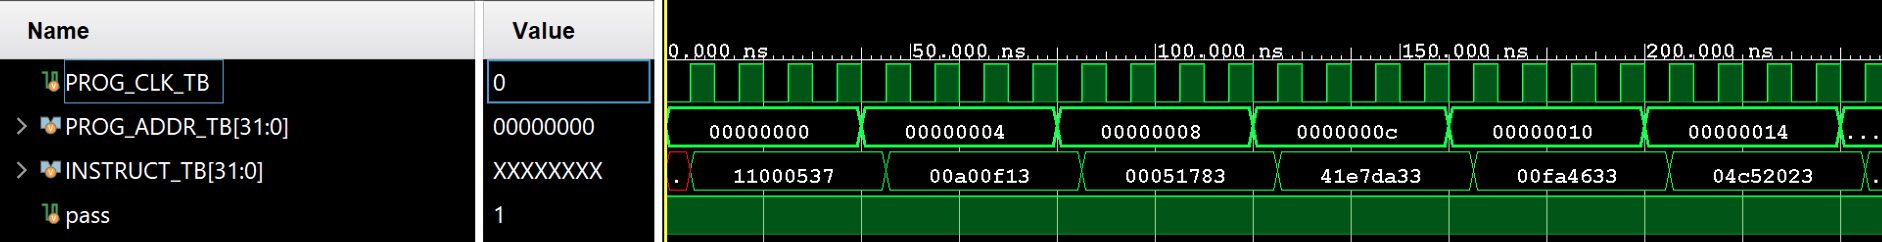
\includegraphics[width=.80\pdfpagewidth]{Figures/ProgRom Simulation.png}
    \caption{ProgRom\_TB Output Waveform}
    \label{fig:ProgRom_TB_Output}
\end{figure}

\section {Conclusion} % Second level section
\hypersetup{urlcolor=blue} 
The ProgRom module was able to be tested and verified to be working correctly. The assembly instructions from the \verb|otter_memory.mem| file were able to be reverse-engineered and then verified by recompiling the assembly instructions and comparing the machine code instructions.
All code for this assignment can be found \href{https://github.com/EthanV1920/CPE-233-Otter/tree/main}{here}.


\end{fullwidth}

% \beg 


%----------------------------------------------------------------------------------------

\end{document}
